\chapter{Work of Last Semester}
\pagenumbering{arabic}\hspace{3mm}

During $6^{th}$ Semester, I wrote a compiler to compile Tiger to MIPS. Now is my attempt to build upon this compiler, to improve its functionality, efficiency and fix various issues/bugs. Also now instead of MIPS, I'll be compiling to RISC V.

\section{What Was Achieved This Semester}

\begin{enumerate}
  \item Successfully translated compiler functionality from MIPS to RISC V.
    \begin{enumerate} 
      \item Now the compiled code is generated based on RISC V machine and corresponding ISA.
      \item During this process, lots of code refactoring is done along with improvement in time complexity of various intermediate computations. Like instead of finding an element in a list, a red black map is used, etc.  
      \item Files such as \href{https://github.com/sourabh2311/btp/blob/master/Compiler/runtime.s}{runtime.s} and \href{https://github.com/sourabh2311/btp/blob/master/Compiler/riscframe.sml}{riscframe.sml} were completely rewritten along with various modifications required at other places.
    \end{enumerate}
  \item Implemented improvements in lexical phase to detect more errors; errors in lexical phase are reported immediately resulting in program termination unlike in semantic analysis where a guess is made to facilitate printing all errors in the end. See figure \ref{fig:lexError} for an example.
    \begin{figure}
    \centering
    \iph{0.80}{assets/lexError.png}
    \caption{Lexer detecting error where newline is inserted in a string}
    \label{fig:lexError}
    \end{figure}
  \item Wrote complete documentation of my compiler at \href{https://tigercompiler.ml}{tigercompiler.ml}. This is done to help me and anyone interested in this project to quickly revise the fundamentals and understand the working of this compiler. Figure \ref{fig:tigercompiler} shows image of the site.
    \begin{figure}
    \centering
    \iph{0.80}{assets/tigercompiler.png}
    \caption{Website: \href{https://tigercompiler.ml}{tigercompiler.ml}}
    \label{fig:tigercompiler}
    \end{figure}
  \item Wrote automated testing using Travis. See \href{https://travis-ci.org/sourabh2311/btp}{this}. Now I'll be able to see whether my changes don't break the existing functionalities and also it is useful in case someone sends a pull request. Figure \ref{fig:travis} shows my project at Travis.
    \begin{figure}
    \centering
    \iph{0.80}{assets/travis.png}
    \caption{Automated testing using \href{https://travis-ci.org/sourabh2311/btp}{Travis}}
    \label{fig:travis}
    \end{figure}
  \item \textbf{Fixed} a major bug; Initially my compiler supported only fixed number of arguments (same as number of argument registers in the machine). Now this has been extended to support any number of arguments (see fig \ref{fig:gitfunargs}). During this process I have as well figured out how to completely remove \texttt{fp} register as it is as such obsolete. This will be done in future. Figure \ref{fig:funargs} shows an example where a lot many arguments are passed to a function and the last argument is returned.   
    \begin{figure}
    \centering
    \iph{0.80}{assets/funargs.png}
    \caption{As many function arguments possible}
    \label{fig:funargs}
    \end{figure}
    \begin{figure}
    \centering
    \iph{0.80}{assets/gitfunargs.png}
    \caption{Git commit showing addition of this feature}
    \label{fig:gitfunargs}
    \end{figure}
  \item Added 2 more arithmetic operations, viz. \texttt{left shift} and \texttt{right shift}. Figure \ref{fig:shiftoperations} shows an example usage of these operations.
    \begin{figure}
    \centering
    \iph{0.80}{assets/shiftoperations.png}
    \caption{Arithmetic Shift Operations}
    \label{fig:shiftoperations}
    \end{figure}
  \item Implemented multiplication by power of 2 optimization inside basic block thus laid foundation for other basic block optimizations like constant propagation, constant folding. An example of multiplication by power of two optimization is shown in figure \ref{fig:mulopt1} and \ref{fig:mulopt2}.
    \begin{figure}[t!]
      \centering
      \begin{subfigure}[t]{\textwidth}
      \centering
      % 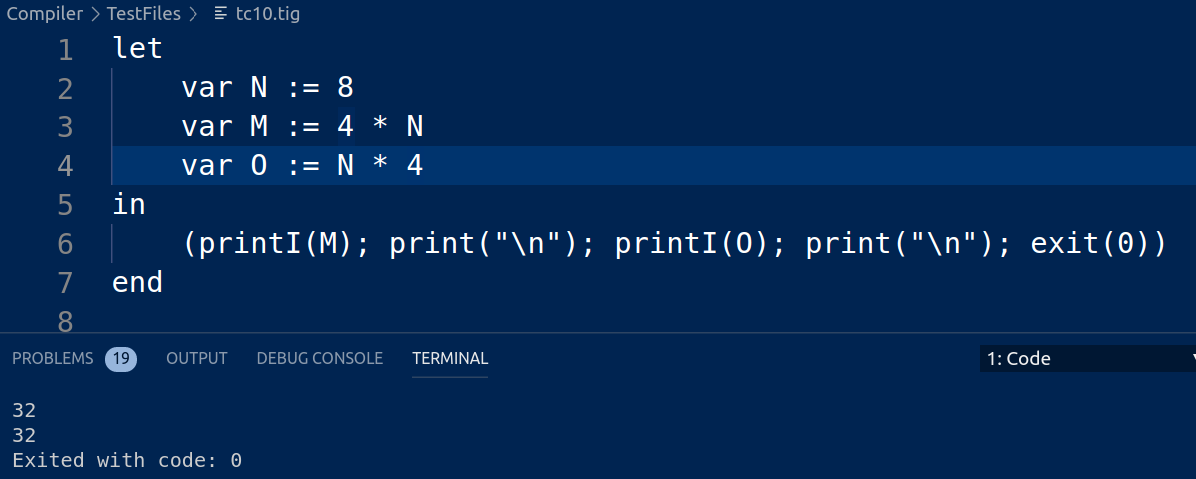
\includegraphics[width=50mm]{assets/mulopt1.png}
      \iph{0.80}{assets/mulopt1.png}
      \caption{Code}
      \label{fig:mulopt1}
      \end{subfigure}
      \begin{subfigure}[t]{0.8\textwidth}
      \centering
      % 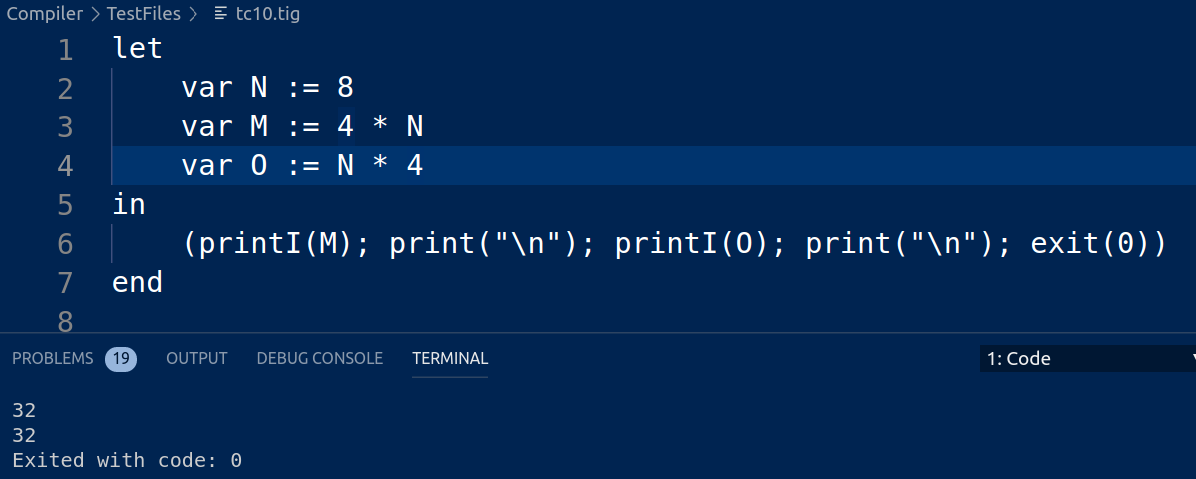
\includegraphics[width=50mm]{assets/mulopt1.png}
      \iph{0.70}{assets/mulopt2.png}
      \caption{\texttt{mul} statements replaced with \texttt{sll}}
      \label{fig:mulopt2}
      \end{subfigure}
      \caption{Multiplication Optimization}
    \end{figure}
  \item Started work on giving a guess of literal in case of small typo. 
  \begin{itemize}
    \item Thinking of printing suggestions which are atmost 2 \href{https://en.wikipedia.org/wiki/Edit_distance}{distance} apart. This will bring the time complexity of standard DP approach of $O(n^2)$ to just $O(n)$. 
    \item Currently the issue is that to implement this, I would have to do lots of modification of the current code. Although I have \href{https://github.com/sourabh2311/btp/commit/8f27478a3c51b9e41bef68961a28c400d4ef29dd}{abstracted} out \textit{Not Found} error messages out with the environment, what is just left is to compare the literal with those of nearby length in the environment. 
    \item But to efficiently get those strings of nearby length there should be a map which maps lengths to the string set. (An array indexed by length may as well be used) To do this, I would have to define additional data structures and put them at appropriate place. 
    \item The main issue is that in the current design, environment just have integers mapped to environment entry. We got this integer by mapping string to counter, not storing the reverse map. This can be worked around by using \href{http://www.cs.utah.edu/~mjones/sml-nj-lib/atom.html}{Atom}.  
  \end{itemize}
  \item Started work on improving my Register Allocator. Current version is a bit simplified version of the algorithm mentioned in the text and is without coalescing.
\end{enumerate}

\section{Road Ahead}

Some among many possible improvements are mentioned below:-

\begin{itemize}
  \item Current implementation of register allocation isn't completely as what is given in the book. My register allocator lacks coalescing and is therefore incomplete. This algorithm was written in hurry last semester and is to be implemented with better heuristics.
  \item Basic blocks has to optimized with optimizations like constant propagation, constant folding, strength reduction etc.
  \item Error messages has to improved in semantic phase. Possible improvement can be to give suggestion for basic typos. 
  \item String comparison has to be made as simple as "str1 $>$ str2", etc.,  instead of calling the string comparison functions to determine it.
  \item To implement ability to include pre-written code (header) files.
  \item To implement garbage collection.
  \item To implement dataflow analyses such as reaching definitions and available expressions and use them to implement some of the optimizations. 
  \item To implement first-class function values in Tiger, so that functions can be passed as arguments and returned as results.
  \item Add support for compile time (initial) arguments.
  \item Implement floating point support.
  \item And much more is possible, its like in a product.
\end{itemize}
